\documentclass{article}

\usepackage[T1]{fontenc} 
\usepackage[utf8]{inputenc}
\usepackage[francais]{babel}
\usepackage{graphicx}

\title{Raport Projet Programmation}
\author{Groupe A : Ali Cherifi, Valentin Gaillard, Julien Pilleux}
\date{23/04/2016}

\begin{document}
\maketitle

\newpage

\section {Les objectifs}
\subsection {Objectifs atteints}
Ali
\subsection {Objectifs non atteints}
Ali

\section {Problème technique}
\subsection {L'affichage dans le terminal}
Au moment d'afficher notre jeu dans le terminal, nous avons cherché à avoir une grille et des instructions les plus propres possibles. Nous avons déjà eu recours au printf classique, mais l'affichage se faisais en dessous et s'empilait ainsi dans le terminal. Celà ne nous convenait pas alors nous avons entendu parlé d'une méthode nous permettant de réafficher par dessus ce que nous avons déjà inscrit. Il fallait toujours utiliser printf mais avec des paramètres supplémentaires au début de celle-ci.
\subsection {Les paramètres de la fonction printf}

\begin{flushleft}

\includegraphics[scale=0.45]{printf_capture.png}
\end{flushleft}

Ce paramètre additionnel nous a permi de pouvoir choisir, directement dans le terminal, où écrire. Le premier paramètre entier, nous permet de choisir quelle est la ligne du terminal nous allons écrire, la ligne est choisie à partir de la vu courante, elle est donc comptée depuis la première ligne affichée du terminal. Ici la variable instruction line correspond à la ligne en dessous de la grille. Un autre problème rencontré est que à chaque affichage de la grille, la vue courrante du terminal changeait, donc pour avoir toujours la même ligne a chaque tour de boucle, il a juste fallut ajouter une fonction permettant de clean l'affichage du terminal (System (``clear'')).
Le second paramètre entier correspond tout simplement au nombre de caractère qu'il faut laisser entre le bord gauche du terminal et le premier caractère de la chaîne de caractère que l'on veut afficher. Ici, le fait de mettre 0 permet de coller la chaîne au bord du terminal.
Finalement, le dernier paramètre, la chaîne de caractère est tout simplement la chaîne à afficher aux coordonnées précédemment choisies. Avec ceci, nous obtenons un affichage propre.

\newpage

\subsection {Le retour à la ligne du prompt}
Même avec ce printf, il nous restait le soucis du prompt qui revenait à la ligne, et les options saisies ne s'affichait pas sur la même ligne. En effet, une fois une option saisie, le curseur se positionnait automatiquement sur la ligne d'en dessous. Pour palier à ça, il a fallut créer une fonction reset cursor qui replaçait le prompt sur la bonne ligne.

\begin{flushleft}
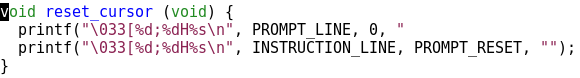
\includegraphics[scale=0.45]{reset_cursor.png}
\end{flushleft}

Cette fonction utilise le printf précédemment vu. Le premier printf sert à réinitialiser la ligne de saisie afin qu'elle apparaisse vide, pour que la prochaine saisie puisse être entrée sans chevauchement de caractères. Puis, la seconde instruction nous sert à imprimer une chaîne de caractère vide sur la ligne au dessus de la ligne de la saisie, pour que le curseur se positionne automatiquement sur cette dernière.

\section {Redondance de code}
Valentin

\end{document}
